\documentclass{article}

\usepackage{arxiv}

\usepackage[utf8]{inputenc} % allow utf-8 input
\usepackage[T1]{fontenc}    % use 8-bit T1 fonts
\usepackage{lmodern}        % https://github.com/rstudio/rticles/issues/343
\usepackage{hyperref}       % hyperlinks
\usepackage{url}            % simple URL typesetting
\usepackage{booktabs}       % professional-quality tables
\usepackage{amsfonts}       % blackboard math symbols
\usepackage{nicefrac}       % compact symbols for 1/2, etc.
\usepackage{microtype}      % microtypography
\usepackage{lipsum}
\usepackage{graphicx}

\title{The spread of COVID-19 in a landlocked country the case of
Luxembourg}

\author{
    Bruno Rodrigues
    \thanks{This preprint was written during my free time as a private
citizen, and reflects in no manner the views of the Ministry of Higher
Education and Research, nor the Government of the Grand-Duchy of
Luxembourg.}
   \\
    Statistics department \\
    Ministry of Higher Education and Research, Grand-Duchy of
Luxembourg \\
  Luxembourg, 18-20, Montée de la Pétrusse \\
  \texttt{\href{mailto:bruno.rodrigues@mesr.etat.lu}{\nolinkurl{bruno.rodrigues@mesr.etat.lu}}} \\
  }

\usepackage{color}
\usepackage{fancyvrb}
\newcommand{\VerbBar}{|}
\newcommand{\VERB}{\Verb[commandchars=\\\{\}]}
\DefineVerbatimEnvironment{Highlighting}{Verbatim}{commandchars=\\\{\}}
% Add ',fontsize=\small' for more characters per line
\usepackage{framed}
\definecolor{shadecolor}{RGB}{248,248,248}
\newenvironment{Shaded}{\begin{snugshade}}{\end{snugshade}}
\newcommand{\AlertTok}[1]{\textcolor[rgb]{0.94,0.16,0.16}{#1}}
\newcommand{\AnnotationTok}[1]{\textcolor[rgb]{0.56,0.35,0.01}{\textbf{\textit{#1}}}}
\newcommand{\AttributeTok}[1]{\textcolor[rgb]{0.77,0.63,0.00}{#1}}
\newcommand{\BaseNTok}[1]{\textcolor[rgb]{0.00,0.00,0.81}{#1}}
\newcommand{\BuiltInTok}[1]{#1}
\newcommand{\CharTok}[1]{\textcolor[rgb]{0.31,0.60,0.02}{#1}}
\newcommand{\CommentTok}[1]{\textcolor[rgb]{0.56,0.35,0.01}{\textit{#1}}}
\newcommand{\CommentVarTok}[1]{\textcolor[rgb]{0.56,0.35,0.01}{\textbf{\textit{#1}}}}
\newcommand{\ConstantTok}[1]{\textcolor[rgb]{0.00,0.00,0.00}{#1}}
\newcommand{\ControlFlowTok}[1]{\textcolor[rgb]{0.13,0.29,0.53}{\textbf{#1}}}
\newcommand{\DataTypeTok}[1]{\textcolor[rgb]{0.13,0.29,0.53}{#1}}
\newcommand{\DecValTok}[1]{\textcolor[rgb]{0.00,0.00,0.81}{#1}}
\newcommand{\DocumentationTok}[1]{\textcolor[rgb]{0.56,0.35,0.01}{\textbf{\textit{#1}}}}
\newcommand{\ErrorTok}[1]{\textcolor[rgb]{0.64,0.00,0.00}{\textbf{#1}}}
\newcommand{\ExtensionTok}[1]{#1}
\newcommand{\FloatTok}[1]{\textcolor[rgb]{0.00,0.00,0.81}{#1}}
\newcommand{\FunctionTok}[1]{\textcolor[rgb]{0.00,0.00,0.00}{#1}}
\newcommand{\ImportTok}[1]{#1}
\newcommand{\InformationTok}[1]{\textcolor[rgb]{0.56,0.35,0.01}{\textbf{\textit{#1}}}}
\newcommand{\KeywordTok}[1]{\textcolor[rgb]{0.13,0.29,0.53}{\textbf{#1}}}
\newcommand{\NormalTok}[1]{#1}
\newcommand{\OperatorTok}[1]{\textcolor[rgb]{0.81,0.36,0.00}{\textbf{#1}}}
\newcommand{\OtherTok}[1]{\textcolor[rgb]{0.56,0.35,0.01}{#1}}
\newcommand{\PreprocessorTok}[1]{\textcolor[rgb]{0.56,0.35,0.01}{\textit{#1}}}
\newcommand{\RegionMarkerTok}[1]{#1}
\newcommand{\SpecialCharTok}[1]{\textcolor[rgb]{0.00,0.00,0.00}{#1}}
\newcommand{\SpecialStringTok}[1]{\textcolor[rgb]{0.31,0.60,0.02}{#1}}
\newcommand{\StringTok}[1]{\textcolor[rgb]{0.31,0.60,0.02}{#1}}
\newcommand{\VariableTok}[1]{\textcolor[rgb]{0.00,0.00,0.00}{#1}}
\newcommand{\VerbatimStringTok}[1]{\textcolor[rgb]{0.31,0.60,0.02}{#1}}
\newcommand{\WarningTok}[1]{\textcolor[rgb]{0.56,0.35,0.01}{\textbf{\textit{#1}}}}

% Pandoc citation processing
\newlength{\csllabelwidth}
\setlength{\csllabelwidth}{3em}
\newlength{\cslhangindent}
\setlength{\cslhangindent}{1.5em}
% for Pandoc 2.8 to 2.10.1
\newenvironment{cslreferences}%
  {}%
  {\par}
% For Pandoc 2.11+
\newenvironment{CSLReferences}[3] % #1 hanging-ident, #2 entry spacing
 {% don't indent paragraphs
  \setlength{\parindent}{0pt}
  % turn on hanging indent if param 1 is 1
  \ifodd #1 \everypar{\setlength{\hangindent}{\cslhangindent}}\ignorespaces\fi
  % set entry spacing
  \ifnum #2 > 0
  \setlength{\parskip}{#2\baselineskip}
  \fi
 }%
 {}
\usepackage{calc} % for calculating minipage widths
\newcommand{\CSLBlock}[1]{#1\hfill\break}
\newcommand{\CSLLeftMargin}[1]{\parbox[t]{\csllabelwidth}{#1}}
\newcommand{\CSLRightInline}[1]{\parbox[t]{\linewidth - \csllabelwidth}{#1}}
\newcommand{\CSLIndent}[1]{\hspace{\cslhangindent}#1}



\begin{document}
\maketitle

\def\tightlist{}


\begin{abstract}
Enter the text of your abstract here.
\end{abstract}

\keywords{
    blah
   \and
    blee
   \and
    bloo
   \and
    these are optional and can be removed
  }

\hypertarget{introduction}{%
\section{Introduction}\label{introduction}}

The Grand-Duchy of Luxembourg is a country that is unique in many ways.
As its official name quite clearly indicates, it is a grand duchy, the
last of its kind on earth. It is a relatively young country, as it
became a grand duchy once it gained independence from Napoleonic France
in 1815 (but was pretty much still a puppet state of the Kingdom of the
Netherlands until the end of the 19th century), is one of the founding
members of the European Coal and Steel Community, which evolved to
become the European Union and has three official languages: French,
German, and Luxembourguish. Luxembourg is also a landlocked country,
sandwiched between France, Germany and Belgium. This geographic position
has given Luxembourg many advantages. One such advantage is that its
labour force, which amounts to 400000 workers and is composed of 50\% of
French, German and Belgian commuters. This is also the reason why
Luxembourg has one of the highest GDPs per capita in the world: half of
its riches are produced by foreigners which are not taken into account
in the computation of GDP per capita.

Half of Luxembourg's population is also composed of foreigners, the
largest community being the Portuguese, followed by the French.

In this article, I posit the following hypothesis: due to its quite
unique characteristics, the spread of COVID-19 in a landlocked country
like Luxembourg is the exact opposite of the spread of COVID-19 that can
be observed on an island country such as New Zealand, or Madagascar. A
landlocked country like Luxembourg, which is furthermore highly
dependent on foreign workers, has many more difficulties to control the
spread of COVID-19 within its borders. Unlike an island country, a
landlocked country that is highly tied to its neighbours cannot simply
close its borders and put a very hard lockdown in place to control the
pandemic. Or if the landlocked country does that, as soon as it opens
its borders, the disease will start spreading again. To illustrate this
idea, I will discuss how COVID-19 starting spreading, but not only
within the borders of Luxembourg, but rather within the so-called
Greater Region. The Greater Region \emph{a space for cross-border
cooperation in the heart of Europe} and is composed of the Grand-Duchy
of Luxembourg, two Belgian Provinces, two French Départements and two
German Bundesländer.

\begin{figure}
  \centering
  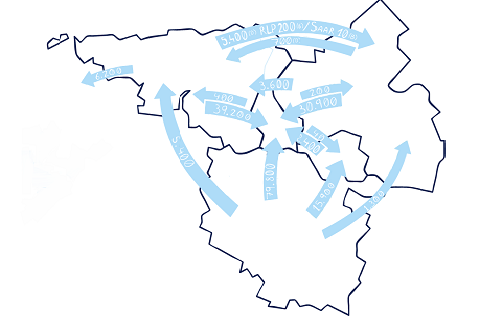
\includegraphics{"~/Documents/covid_grande_region/paper/figs/commuters.png"}
  \caption{The daily commuters in the Greater Region. Luxembourg absorbs the vast majority. (Source: Bienvenue dans la Grande Région, 2018)}
  \label{commuters}
\end{figure}

Figure \ref{commuters} show a map of the Greater Region with the flows
of daily commuters between its constituent regions. Every day, according
to this map from 2018, more than 150000 commuters go to Luxembourg to
work. In 2019, it was reported that this number reached
200000.\footnote{\url{https://paperjam.lu/article/plus-200-000-frontaliers-sur-m}}

The goal of this work is thus as follows: I will train machine learning
models to predict the spread of COVID-19 in Luxembourg using openly
available data on the weekly positive cases of COVID-19. However,
because of the very tight economic and social integration of Luxembourg
to its neighbours I will use as features weekly positive cases in the
border regions as well as Google Mobility
data\footnote{\url{https://www.google.com/covid19/mobility/}} for
Luxembourg to proxy for hard, and soft, lockdowns. I will show that
weekly, and most importantly lags of weekly cases in the neighbouring
regions predict cases for Luxembourg.

\hypertarget{the-covid-19-pandemic-in-the-greater-region}{%
\section{The COVID-19 pandemic in the Greater
Region}\label{the-covid-19-pandemic-in-the-greater-region}}

\begin{Shaded}
\begin{Highlighting}[]
\FunctionTok{tar\_read}\NormalTok{(epid\_curves)}
\end{Highlighting}
\end{Shaded}

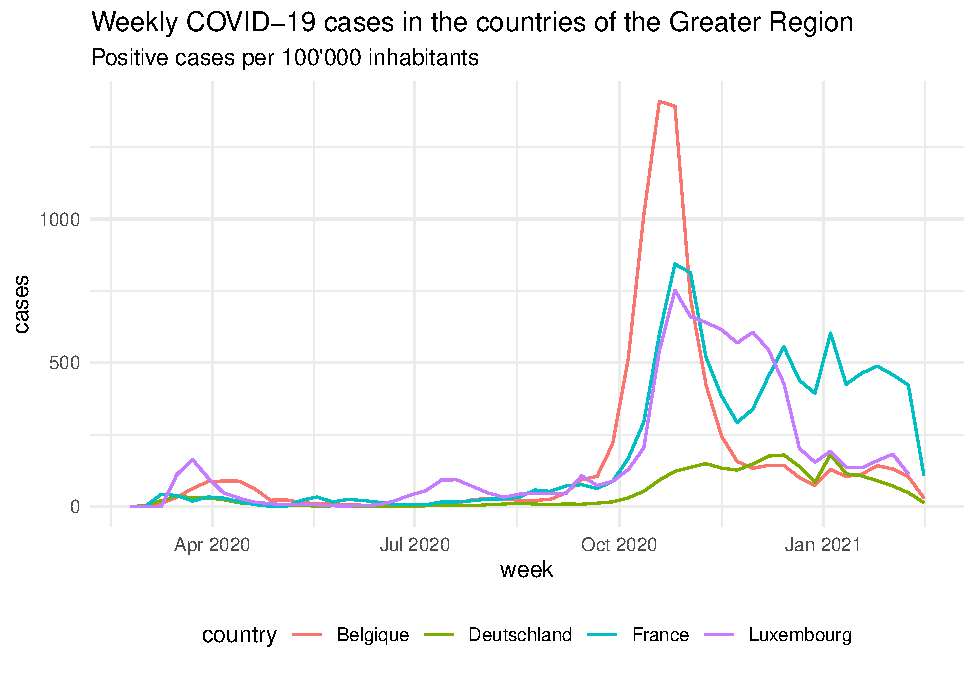
\includegraphics{paper_files/figure-latex/unnamed-chunk-1-1.pdf}

\begin{Shaded}
\begin{Highlighting}[]
\FunctionTok{tar\_read}\NormalTok{(epidem\_map)}\SpecialCharTok{$}\NormalTok{map\_first\_wave}
\end{Highlighting}
\end{Shaded}

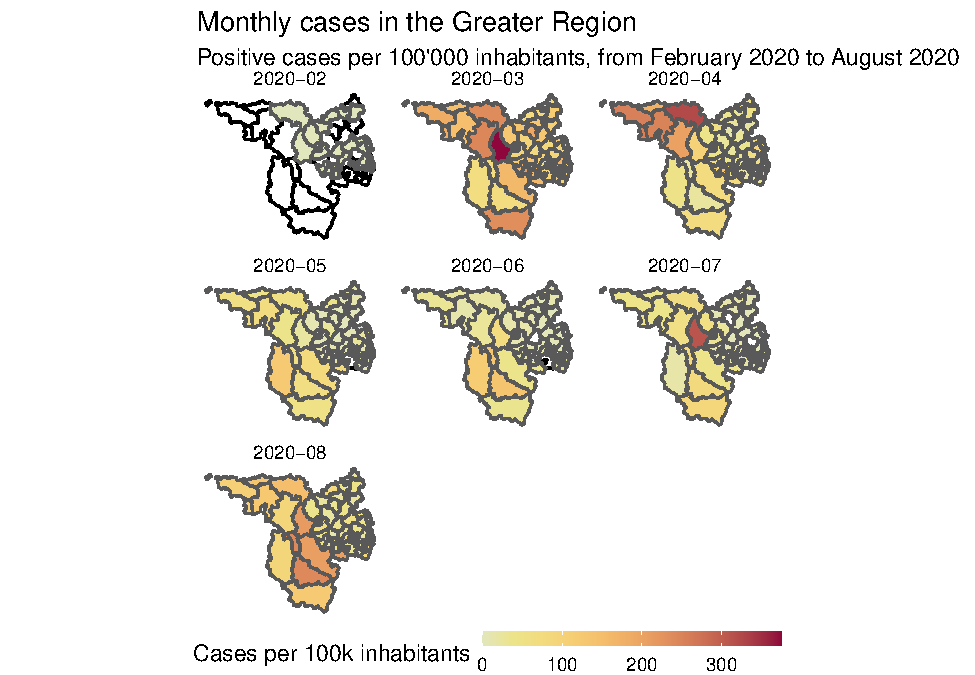
\includegraphics[width=1\linewidth]{paper_files/figure-latex/unnamed-chunk-2-1}

\begin{Shaded}
\begin{Highlighting}[]
\FunctionTok{tar\_read}\NormalTok{(epidem\_map)}\SpecialCharTok{$}\NormalTok{map\_second\_wave}
\end{Highlighting}
\end{Shaded}

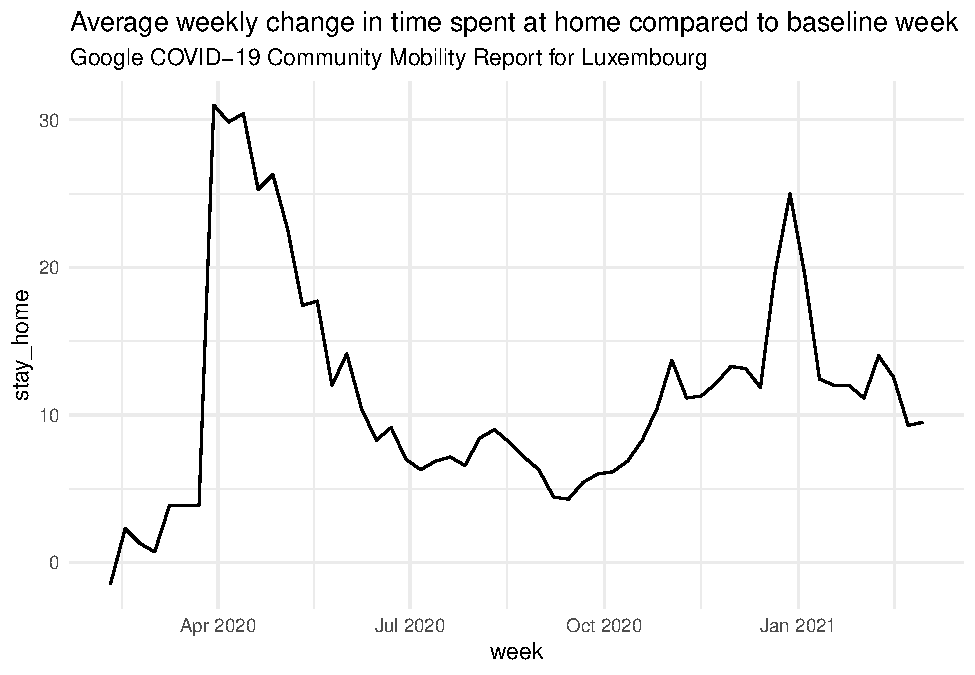
\includegraphics[width=1\linewidth]{paper_files/figure-latex/unnamed-chunk-3-1}

\begin{Shaded}
\begin{Highlighting}[]
\FunctionTok{tar\_read}\NormalTok{(cv\_plan)}
\end{Highlighting}
\end{Shaded}

\begin{verbatim}
## Warning: Removed 1 row(s) containing missing values (geom_path).
\end{verbatim}

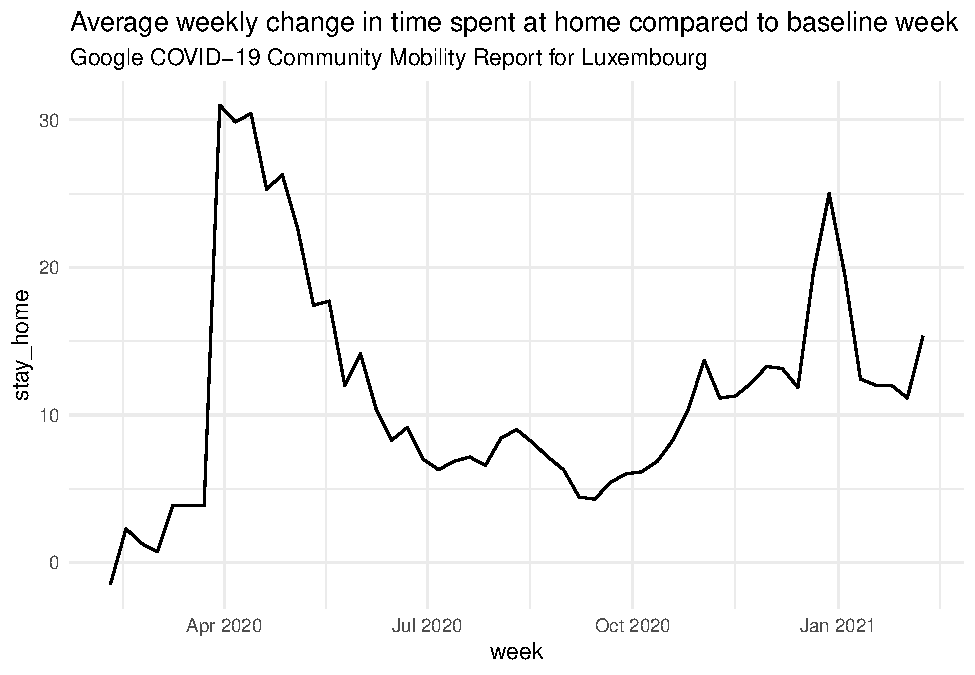
\includegraphics{paper_files/figure-latex/unnamed-chunk-4-1.pdf}

\begin{Shaded}
\begin{Highlighting}[]
\FunctionTok{tar\_read}\NormalTok{(forecast\_plot)}
\end{Highlighting}
\end{Shaded}

\begin{verbatim}
## Warning in max(ids, na.rm = TRUE): no non-missing arguments to max; returning
## -Inf

## Warning in max(ids, na.rm = TRUE): no non-missing arguments to max; returning
## -Inf

## Warning in max(ids, na.rm = TRUE): no non-missing arguments to max; returning
## -Inf

## Warning in max(ids, na.rm = TRUE): no non-missing arguments to max; returning
## -Inf

## Warning in max(ids, na.rm = TRUE): no non-missing arguments to max; returning
## -Inf
\end{verbatim}

\begin{verbatim}
## Warning: Removed 1 row(s) containing missing values (geom_path).
\end{verbatim}

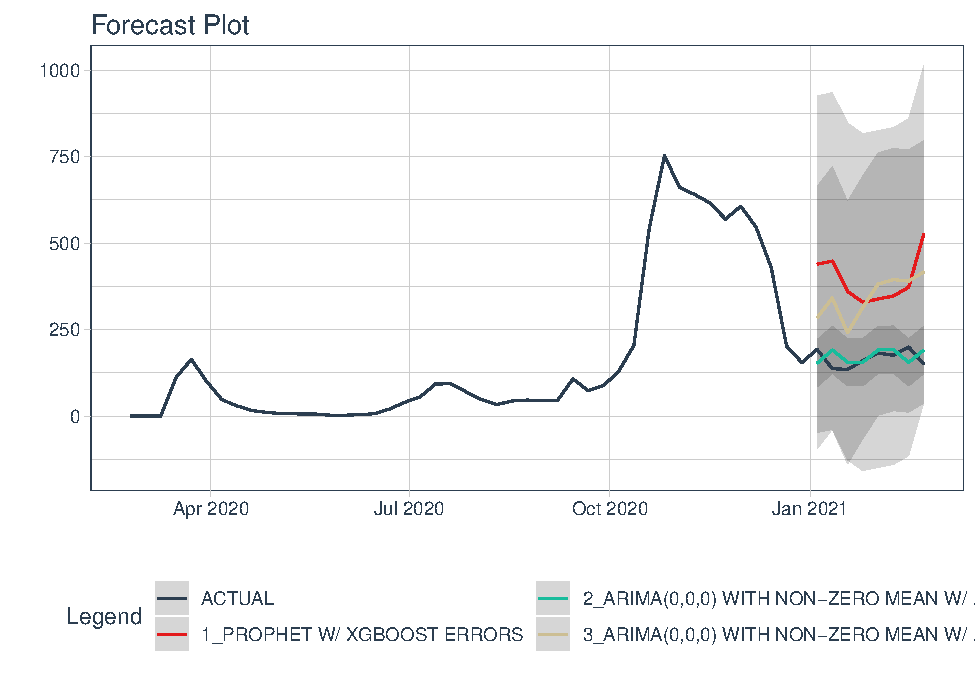
\includegraphics{paper_files/figure-latex/unnamed-chunk-5-1.pdf}

\hypertarget{headings-first-level}{%
\section{Headings: first level}\label{headings-first-level}}

\label{sec:headings}

\lipsum[4] See Section \ref{sec:headings}.

\hypertarget{headings-second-level}{%
\subsection{Headings: second level}\label{headings-second-level}}

\lipsum[5]

\[
\xi _{ij}(t)=P(x_{t}=i,x_{t+1}=j|y,v,w;\theta)= {\frac {\alpha _{i}(t)a^{w_t}_{ij}\beta _{j}(t+1)b^{v_{t+1}}_{j}(y_{t+1})}{\sum _{i=1}^{N} \sum _{j=1}^{N} \alpha _{i}(t)a^{w_t}_{ij}\beta _{j}(t+1)b^{v_{t+1}}_{j}(y_{t+1})}}
\]

\hypertarget{headings-third-level}{%
\subsubsection{Headings: third level}\label{headings-third-level}}

\lipsum[6]

\paragraph{Paragraph}
\lipsum[7]

\hypertarget{examples-of-citations-figures-tables-references}{%
\section{Examples of citations, figures, tables,
references}\label{examples-of-citations-figures-tables-references}}

\label{sec:others}

\lipsum[8] some text (Kour and Saabne 2014b, 2014a) and see Hadash et
al. (2018).

The documentation for \verb+natbib+ may be found at

\begin{center}
  \url{http://mirrors.ctan.org/macros/latex/contrib/natbib/natnotes.pdf}
\end{center}

Of note is the command \verb+\citet+, which produces citations
appropriate for use in inline text. For example,

\begin{verbatim}
   \citet{hasselmo} investigated\dots
\end{verbatim}

produces

\begin{quote}
  Hasselmo, et al.\ (1995) investigated\dots
\end{quote}

\begin{center}
  \url{https://www.ctan.org/pkg/booktabs}
\end{center}

\hypertarget{figures}{%
\subsection{Figures}\label{figures}}

\lipsum[10] See Figure \ref{fig:fig1}. Here is how you add footnotes.
{[}\^{}Sample of the first footnote.{]}

\lipsum[11]

\begin{figure}
  \centering
  \fbox{\rule[-.5cm]{4cm}{4cm} \rule[-.5cm]{4cm}{0cm}}
  \caption{Sample figure caption.}
  \label{fig:fig1}
\end{figure}

\begin{Shaded}
\begin{Highlighting}[]
\FunctionTok{plot}\NormalTok{(mtcars}\SpecialCharTok{$}\NormalTok{mpg)}
\end{Highlighting}
\end{Shaded}

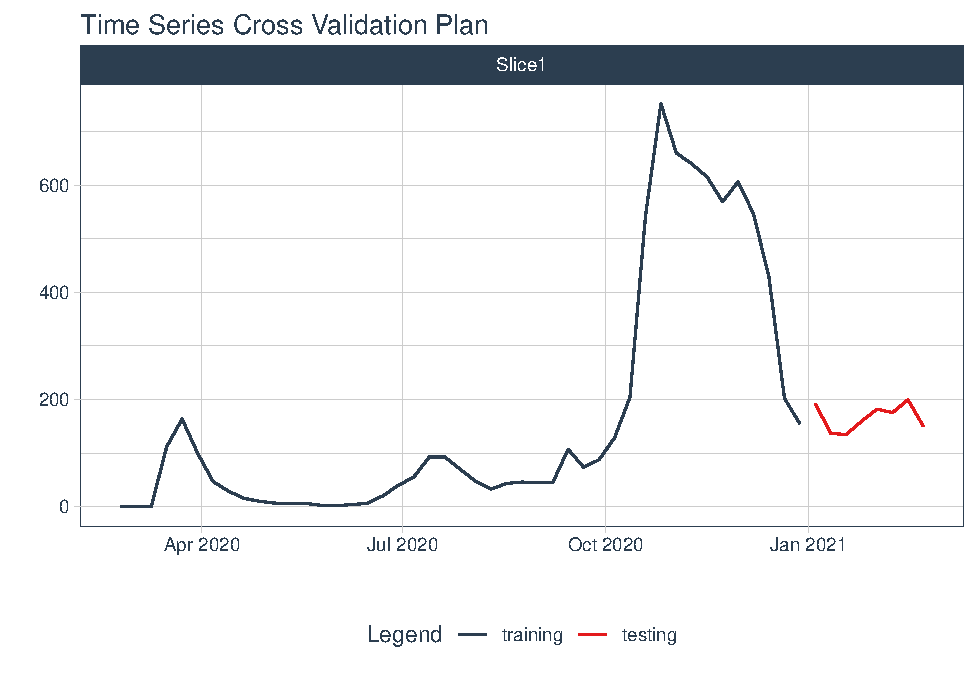
\includegraphics{paper_files/figure-latex/unnamed-chunk-6-1.pdf}

\hypertarget{tables}{%
\subsection{Tables}\label{tables}}

\lipsum[12]

See awesome Table\textasciitilde{}\ref{tab:table}.

\begin{table}
 \caption{Sample table title}
  \centering
  \begin{tabular}{lll}
    \toprule
    \multicolumn{2}{c}{Part}                   \\
    \cmidrule(r){1-2}
    Name     & Description     & Size ($\mu$m) \\
    \midrule
    Dendrite & Input terminal  & $\sim$100     \\
    Axon     & Output terminal & $\sim$10      \\
    Soma     & Cell body       & up to $10^6$  \\
    \bottomrule
  \end{tabular}
  \label{tab:table}
\end{table}

\hypertarget{lists}{%
\subsection{Lists}\label{lists}}

\begin{itemize}
\tightlist
\item
  Lorem ipsum dolor sit amet
\item
  consectetur adipiscing elit.
\item
  Aliquam dignissim blandit est, in dictum tortor gravida eget. In ac
  rutrum magna.
\end{itemize}

\hypertarget{refs}{}
\begin{CSLReferences}{1}{0}
\leavevmode\hypertarget{ref-hadash2018estimate}{}%
Hadash, Guy, Einat Kermany, Boaz Carmeli, Ofer Lavi, George Kour, and
Alon Jacovi. 2018. {``Estimate and Replace: A Novel Approach to
Integrating Deep Neural Networks with Existing Applications.''}
\emph{arXiv Preprint arXiv:1804.09028}.

\leavevmode\hypertarget{ref-kour2014fast}{}%
Kour, George, and Raid Saabne. 2014a. {``Fast Classification of
Handwritten on-Line Arabic Characters.''} In \emph{Soft Computing and
Pattern Recognition (SoCPaR), 2014 6th International Conference of},
312--18. IEEE.

\leavevmode\hypertarget{ref-kour2014real}{}%
---------. 2014b. {``Real-Time Segmentation of on-Line Handwritten
Arabic Script.''} In \emph{Frontiers in Handwriting Recognition (ICFHR),
2014 14th International Conference on}, 417--22. IEEE.

\end{CSLReferences}

\bibliographystyle{unsrt}
\bibliography{references.bib}


\end{document}
